\documentclass[aspectratio=169,compress]{beamer}
  \useoutertheme[footline=authorinstitute,subsection=false]{miniframes}
  \useinnertheme{circles}
  \usefonttheme{default}

  \definecolor{palatinate}{RGB}{126,49,123}
  \definecolor{pale-palatinate}{RGB}{216,172,214}
  \definecolor{grey-palatinate}{RGB}{150,142,133}
  \definecolor{dirt-palatinate}{RGB}{159,161,97}
  \definecolor{blue-palatinate}{RGB}{0,99,136}

  \setbeamercolor*{palette primary}{fg=blue-palatinate}
  \setbeamercolor*{palette secondary}{fg=palatinate,bg=pale-palatinate}
  \setbeamercolor*{palette tertiary}{fg=white,bg=palatinate}
  \setbeamercolor*{palette quaternary}{fg=white,bg=dirt-palatinate}

  \setbeamercolor*{normal text}{parent=palette primary}
  \setbeamercolor*{footline}{parent=palette secondary}
  \setbeamercolor*{headline}{parent=palette tertiary}
  \setbeamercolor*{titlelike}{parent=palette secondary}

  \setbeamercolor*{structure}{parent=normal text}
  \setbeamercolor*{title in head/foot}{parent=headline}
  \setbeamercolor*{section in head/foot}{parent=headline}
  \setbeamercolor*{author in head/foot}{parent=footline}
  \setbeamercolor*{institute in head/foot}{parent=footline}

  \setbeamercolor*{alerted text}{parent=normal text,fg=palatinate}

  \setbeamercolor*{block title}{fg=white,bg=blue-palatinate}
  \setbeamercolor*{block body}{parent=normal text,bg=pale-palatinate!5}

  \setbeamercolor*{block title example}{fg=white,bg=dirt-palatinate}
  \setbeamercolor*{block body example}{parent=normal text,bg=dirt-palatinate!5}

  \setbeamertemplate{bibliography item}[text]
  \setbeamertemplate{blocks}[rounded][shadow=true]
  \setbeamertemplate{caption}[numbered]
  \setbeamertemplate{frametitle}[default][wd=\textwidth]
  % \setbeamertemplate{navigation symbols}{}
  \setbeamertemplate{title page}[default][rounded=true,shadow=true]

  \setbeamerfont{block title}{size=\small}

  \BeforeBeginEnvironment{frame}{\citereset}
\usepackage[bibstyle=science,citestyle=numeric-comp]{biblatex}
  \bibliography{references.bib}
\usepackage[%
  format=hang,
  labelfont={footnotesize,bf},
  textfont={footnotesize,it}
]{caption}
\usepackage{hyperref}
\usepackage[utf8]{inputenc}
\usepackage{multicol}
\usepackage{siunitx}
\usepackage{tikz}
  \usetikzlibrary{calc}
  \usetikzlibrary{external}
    \tikzexternalize[prefix=tikz/]
  \usetikzlibrary{positioning}
  \usetikzlibrary{shapes.geometric}
  \usetikzlibrary{shapes.misc}
  \usetikzlibrary{fadings}

  \newcommand\pgfmathsinandcos[3]{%
    \pgfmathsetmacro#1{sin(#3)}%
    \pgfmathsetmacro#2{cos(#3)}%
  }
  \newcommand\LongitudePlane[3][current plane]{%
    \pgfmathsinandcos\sinEl\cosEl{#2} % elevation
    \pgfmathsinandcos\sint\cost{#3} % azimuth
    \tikzset{#1/.style={cm={\cost,\sint*\sinEl,0,\cosEl,(0,0)}}}
  }
  \newcommand\DrawLongitudeArc[2][1]{
    \LongitudePlane{\angEl}{#2}
    \tikzset{current plane/.prefix style={scale=#1}}
     % angle of "visibility"
    % \pgfmathsetmacro\angVis{atan(sin(#2)*cos(\angEl)/sin(\angEl))} %
    \draw[current plane] (90:1) arc (90:270:1);
    % \draw[current plane,dashed] (\angVis:1) arc (\angVis:\angVis+180:1);
    % \draw[current plane,dashed] (\angVis-180:1) arc (\angVis-180:\angVis:1);
  }
  \newcommand\ClipLongitudeArc[2][1]{
    \LongitudePlane{\angEl}{#2}
    \tikzset{current plane/.prefix style={scale=#1}}
    \clip[current plane] (90:1) arc (90:270:1);
  }

\renewcommand*{\footnotefont}{\tiny}
\renewcommand*{\bibfont}{\tiny}
\newcommand*{\autotitle}{\subsecname\hfill\textbf{\small\secname}}

\author{Russell Maguire}
\title{Nanocarriers for targeted drug delivery}
\subtitle{Benefits and challenges of nanotechnology for medicine}
\institute{ENGI4131 Advanced Semiconductor Devices \and Durham University}
\date{\today}
\logo{\Large\includegraphics[height=1em]{img/Durham.png}}

\begin{document}

\frame{\titlepage}

% \section*{Outline}
% \frame{\tableofcontents}

\section{Introduction}

\subsection{Nanocarrier delivery systems}
\begin{frame}[fragile]{\autotitle}
  \begin{columns}
    \column{0.5\textwidth}
      \begin{block}{Nanocarrier structure}
        \begin{figure}
          \small
          \centering
          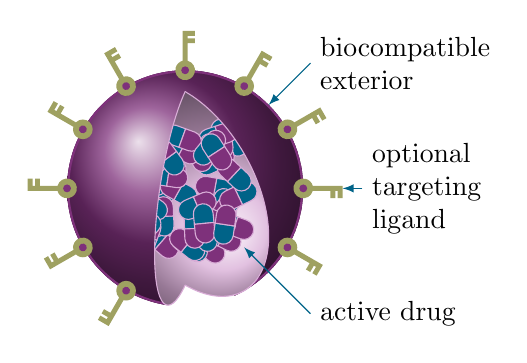
\begin{tikzpicture}[%
            >=latex,
            drug/.pic={%
              \path [draw=pale-palatinate,fill=blue-palatinate] (0,#1/2)
                -- (#1/2,#1/2)
                arc (90:-90:#1/2)
                -- (0,-#1/2)
                -- cycle;
              \path [draw=pale-palatinate,fill=palatinate] (0,-#1/2)
                -- (-#1/2,-#1/2)
                arc (270:90:#1/2)
                -- (0,#1/2)
                -- cycle;
            },
            ligand/.pic={%
              \fill [dirt-palatinate] (15:#1/4) 
                -| (#1,-#1/4)
                -| (#1-#1/8,-#1/4*sin{15})
                -| (#1-1.5*#1/8,-#1/4)
                -- (#1-2.5*#1/8,-#1/4)
                |- (-15:#1/4)
                arc (345:15:#1/4)
                -- cycle;
              \fill [palatinate] (0,0) circle (#1/10);
            }
          ]
            \def\R{1.5}
            \def\angEl{35}
            \def\angLatA{75}
            \def\angLatB{135}

            \begin{scope}
              \clip (0,0)
                -- ({270-\angEl*cos(\angLatA)}:\R)
                arc ({270-\angEl*cos(\angLatA)}:{-90-\angEl*cos(\angLatB)}:\R)
                -- cycle;
              \filldraw [palatinate,ultra thick,ball color=palatinate] (0,0) circle (\R);
            \end{scope}
            \foreach \t in {\angLatA,\angLatB} {%
              \pgfmathsetseed{1234}
              \begin{scope}
                \ClipLongitudeArc[\R]{\t};
                \shade [shading angle=180,ball color=pale-palatinate] (0,0) circle (\R);
                \foreach \i in {1,...,50}
                  \pic [rotate=rand*180] at (rand*\R/2,rand*\R/2) {drug={\R/6}};
              \end{scope}
              \begin{scope}[line cap=round,draw=pale-palatinate]
                  \DrawLongitudeArc[\R]{\t};
              \end{scope}
            }
            \foreach \t in {-30,0,...,240}
              \pic [rotate=\t] at (\t:\R) {ligand=\R/3};
            \node [anchor=west,align=left] (nanoparticle) at (45:1.5*\R) {biocompatible\\exterior};
            \node [anchor=west,align=left] (ligand) at (0:1.5*\R) {optional\\targeting\\ligand};
            \node [anchor=west,align=left] (drug) at (-45:1.5*\R) {active drug};

            \draw [->,blue-palatinate] (nanoparticle.west) -- (45:\R);
            \draw [->,blue-palatinate] (ligand.west) -- (0:4/3*\R);
            \draw [->,blue-palatinate] (drug.west) -- (-45:{\R/sqrt(2)});
          \end{tikzpicture}
        \end{figure}
      \end{block}

    \column{0.5\textwidth}
      \begin{block}{Definition: nanocarrier}
        \begin{itemize}
          \item Biocompatible nanoparticle encapsulating a drug
        \end{itemize}
      \end{block}

      \begin{block}{Characteristics}
        \begin{columns}[t,onlytextwidth]
          \column{0.55\textwidth}\vskip-1em
            \begin{itemize}
              \item \alert{Nanometre scale}
              \item \alert{Biodegradable}
              \item \alert{Non-immunogenic}
            \end{itemize}
          \column{0.45\textwidth}\vskip-1em
            \begin{itemize}
              \item \alert{Low toxicity}
              \item \alert{Hydrophilic}
              \item \alert{Soluble}
            \end{itemize}
        \end{columns}
      \end{block}

  \end{columns}
\end{frame}

\subsection{Targeted drug delivery}
\begin{frame}{\autotitle}
  \begin{columns}

    \column{0.5\textwidth}
      \begin{block}{How is targeted drug delivery effective?}
        \begin{figure}
          \small
          \centering
          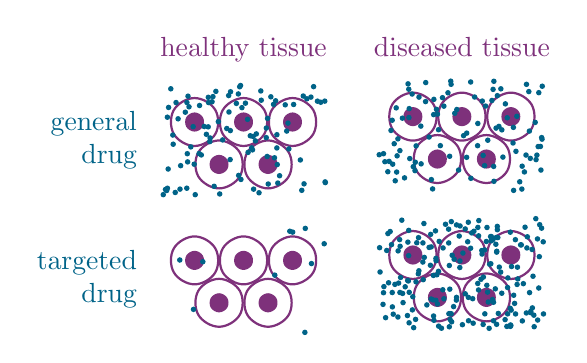
\begin{tikzpicture}[%
            hexagon/.style={regular polygon,regular polygon sides=6},
            cell/.pic={%
              \coordinate (-O) at (0,0);
              \node [%
                thick,
                anchor=center,
                draw,
                hexagon,
                rounded corners=2em/4,
                minimum size=2em,
                inner sep=0pt,
                outer sep=2em/3,
                pic actions,
              ] (-wall) at (-O) {};
              \node [%
                anchor=center,
                fill,
                hexagon,
                rounded corners=0.8em/4,
                minimum size=0.8em,
                inner sep=0pt,
                outer sep=0pt,
                pic actions,
              ] (-nucleus) at (-O) {};
            },
            tissue/.pic={%
              \coordinate (-O) at (0,0);
              \pic (-cell 0) at (0,2em/3) {cell};
              \foreach \i in {3,...,6}
                \pic (-cell \i) at (-cell 0-wall.corner \i) {cell};
            }
          ]
            \node [%
              palatinate,
            ] (healthy) {healthy tissue};
            \coordinate [below=2.5em of healthy] (healthy general);
            \coordinate [below=5em of healthy general] (healthy targeted);
            \pic [palatinate] at (healthy targeted) {tissue};
            \pic [palatinate] at (healthy general) {tissue};
            \foreach \x in {1,...,100}
              \fill [blue-palatinate] ($(1.5*2em*rand,2em*rand)+(healthy general)$) circle (0.1em);
            \foreach \x in {1,...,10}
              \fill [blue-palatinate] ($(1.5*2em*rand,2em*rand)+(healthy targeted)$) circle (0.1em);

            \node [%
              palatinate,
              align=center,
              base right=1em of healthy,
            ] (diseased) {diseased tissue};
            \coordinate [below=2.5em of diseased] (diseased general);
            \coordinate [below=5em of diseased general] (diseased targeted);
            \pic [palatinate] at (diseased targeted) {tissue};
            \pic [palatinate] at (diseased general) {tissue};
            \foreach \x in {101,...,200}
              \fill [blue-palatinate] ($(1.5*2em*rand,2em*rand)+(diseased general)$) circle (0.1em);
            \foreach \x in {11,...,200}
              \fill [blue-palatinate] ($(1.5*2em*rand,2em*rand)+(diseased targeted)$) circle (0.1em);

            \node [%
              blue-palatinate,
              align=right,
              left=3.5em of healthy general,
            ] {general\\drug};
            \node [%
              blue-palatinate,
              align=right,
              left=3.5em of healthy targeted,
            ] {targeted\\drug};
          \end{tikzpicture}
          \caption{Goal is to increase drug concentration ratio for diseased tissue.}
        \end{figure}
      \end{block}

    \column{0.5\textwidth}
      \begin{block}{Targets diseased tissue}
        \begin{itemize}
          \item Maximise therapeutic effects
          \item Minimise effective drug dose
          \item Common targets are \alert{solid~tumours}, \alert{inflamed} and \alert{infected~tissue}
        \end{itemize}
      \end{block}

      \begin{block}{Avoids healthy tissue}
        \begin{itemize}
          \item Minimise toxic side-effects
        \end{itemize}
      \end{block}

  \end{columns}
\end{frame}

\section{Passive targeting}

\subsection{Vascular permeability}
\begin{frame}{\autotitle}
  \begin{columns}
    \column{0.5\textwidth}
    \column{0.5\textwidth}
      \begin{block}{Definition: vascular permeability}
        \begin{itemize}
          \item Tendency for molecules to leak from \alert{blood~vessels} into \alert{interstitial~space} between cells
        \end{itemize}
      \end{block}

      \begin{block}{Contributing factors}
        \begin{itemize}
          \item Permeability enhancers such as \emph{bradykinin} and \emph{nitric oxide}
          \item Dense and defective blood vessels
          \item Enhanced vascular permeability has been observed in \alert{solid~tumours} and \alert{inflamed~tissue}~\footcitemark{maeda2000tumor}
        \end{itemize}
      \end{block}

  \end{columns}
  \footcitetext{maeda2000tumor}
\end{frame}

\subsection{Enhanced permeability and retention effect}
\begin{frame}{\autotitle}
  \begin{columns}
    \column{0.5\textwidth}
      \begin{beamercolorbox}[rounded=true,shadow=true]{titlelike}\small
          Basis for \textbf{first generation} nanomedicines~\footcitemark{wicki2015nanomedicine}
      \end{beamercolorbox}

    \column{0.5\textwidth}
      \begin{block}{Definition: EPR effect}
        \begin{itemize}
          \item Tendency for nanoparticles to accumulate in \alert{solid~tumours}~\footcitemark{maeda2000tumor}
        \end{itemize}
      \end{block}

      \begin{block}{Accumulation procedure}
        \begin{enumerate}
          \item Molecules leak into interstitial space due to \alert{enhanced vascular permeability}
          \item \alert{Lymphatic vessels} are compressed by rapidly growing solid tumour~\footcitemark{padera2004pathology}
          \item Large particles become trapped
        \end{enumerate}
      \end{block}

  \end{columns}
  \footcitetext{maeda2000tumor,wicki2015nanomedicine,padera2004pathology}
\end{frame}

\section{Stimuli-responsive targeting}

\subsection{Internal stimuli-responsive nanocarriers}
\begin{frame}{\autotitle}
  \begin{columns}
    \column{0.5\textwidth}
    \column{0.5\textwidth}
      \begin{block}{Bioindicators used to trigger release}
        \begin{itemize}
          \item Tumours have been observed with lower \alert{pH} than healthy tissue~\footcitemark{tannock1989acid,gerweck1996cellular}
          \item Individual organelles maintain their own unique pH and \alert{redox potential}
          \item Intracellular and extracellular space maintain different redox potentials~\textbf{\footcitemark{saito2003drug}}
        \end{itemize}
      \end{block}

  \end{columns}
  \footcitetext{gerweck1996cellular,tannock1989acid,saito2003drug}
\end{frame}

\subsection{External stimuli-responsive nanocarriers}
\begin{frame}{\autotitle}
  \begin{columns}
    \column{0.5\textwidth}
    \column{0.5\textwidth}
      \begin{block}{Mechanisms used to externally trigger release}
        \begin{columns}[t,onlytextwidth]
          \column{0.65\textwidth}\vskip-1em
            \begin{itemize}
              \item \alert{Electromagnetic fields}
              \item \alert{Ultrasound}
            \end{itemize}
          \column{0.35\textwidth}\vskip-1em
            \begin{itemize}
              \item \alert{Heat}
              \item \alert{Light}
            \end{itemize}

        \end{columns}
      \end{block}
  \end{columns}
\end{frame}

\section{Active targeting}

\subsection{Surface ligands}

\begin{frame}{\autotitle}
  \begin{columns}
    \column{0.5\textwidth}
    \column{0.5\textwidth}
      \begin{block}{Definition: active targeting} 
      \end{block}

  \end{columns}
\end{frame}

\begin{frame}
  \begin{beamercolorbox}[rounded=true,shadow=true,sep=8pt]{titlelike}\centering\Large
    Thank you, any questions?
  \end{beamercolorbox}
  \vfill
  \begin{block}{References}\bibfont
    \begin{multicols*}{2}[\vskip-1em]
      \printbibliography
    \end{multicols*}
  \end{block}
\end{frame}

\end{document}
